\chapter{Herramientas Software utilizadas}\label{cap:herramientas}

 En este capítulo, se explicarán las herramientas software utilizadas para llevar a cabo este TFG, es decir, se comentarán los recursos que han servido para la programación y estructuración del proyecto.

\section{Ecosistema: Middleware ROS 2}

ROS\footnote{\url{https://www.ros.org/}} es un middleware que ofrece un conjunto de bibliotecas y herramientas de software que ayudan a crear aplicaciones robóticas. Desde controladores hasta algoritmos de vanguardia, y con potentes herramientas de desarrollo, tiene todo lo necesario para consruir un proyecto de robótica. Y todo es de código abierto.

Tiene dos versiones, ROS (también conocida cómo ROS1, es la primera que salió y la más antigua) y ROS2, la más moderna y la que ha sido utilizada para este proyecto. Además de ser el middleware por excelencia utilizado a lo largo de la carrera por diferentes asignaturas, ROS2 es una potente herramienta utilizada alrededor del mundo para manejar robots.

Dispone de varias distribuciones que van saliendo cada cierto tiempo, cada una compatible con una distribución de Ubuntu concreta. En mi caso, se ha utilizado la anterior dsitribución de ROS2, Humble Hawksbill\footnote{\url{https://docs.ros.org/en/humble/Installation.html}}, debido a que la distribución Ubuntu utilizada ha sido la 22.04 LTS, distribución directamente compatible con Humble.

Para trabajar con ROS, es necesario crear paquetes \cite{tutorial_paquete} para alojar los diferentes programas para publicar o suscribirse a los \textit{topics} del robot \cite{tutorial_pubsub} y especificaciones necesarias para tu aplicación robótica, y pueden crearse directamente para los lenguajes C++, o Python, de los cuales se ha optado por el segundo.

\section{Lenguaje de programación: Python}

Como bien se ha dicho anteriormente, el lenguaje de programación utilizado ha sido Python\footnote{\url{https://www.python.org/}}, lenguaje de alto nivel de programación interpretado cuya filosofía hace hincapié en la legibilidad de su código. Se trata de un lenguaje de programación multiparadigma, ya que soporta parcialmente la orientación a objetos, programación imperativa y, en menor medida, programación funcional. Es un lenguaje interpretado, dinámico y multiplataforma.

Se ha optado por este lenguaje ya que está ampliamente extendido y es fácil de interpretar y utilizar, además de que es compatible con ROS2, pudiendo crear paquetes directamente para este lenguaje. La versión utilizada ha sido la 3.10, versión por defecto instalada en Ubuntu 22.04.

\section{Simulador Gazebo}

Una vez elegidos el middleware y el lenguaje de programación, es necesario elegir un robot y un escenario. Cómo adquirir un robot es algo costoso y mi situación personal no permitía trabajar con los robots que ofrece nuestro laboratorio en la URJC, se optó por trabajar en un entorno completamente simulado.

Para ello, Gazebo\footnote{\url{https://gazebosim.org/home}} fue la mejor opción, por su directa compatibilidad con ROS2 y potencia de simulación, además de que, como ROS, es de código abierto.

A la hora de elegir la versión a utilizar, se decidió usar la versión más reciente del simulador, Gazebo Harmonic, para así no quedarnos tan atrás a la hora de desarrollar, ya que usábamos la versión anterior de ROS2.

\subsection{Modelo del robot NAO simulado}

Una vez escogido el entorno de simulación, era hora de buscar un robot adecuado para el proyecto. Como ya se ha mencionado, nuestro protagonista es el Robot NAO, de Aldebaran, por lo que era necesario encontrar un modelo en el formato de Gazebo (SDF) para poder hacerlo funcionar.

Para esto, Gazebo dispone de una amplia biblioteca\footnote{\url{https://app.gazebosim.org/dashboard}} de mundos y modelos ya creados por empresas o la comunidad, así que sólo era buscarlo en esta biblioteca.

Al final, el modelo utilizado sería el ofrecido por OpenRobotics, que se muestra a continuación:

\begin{figure}[H]
    \centering
    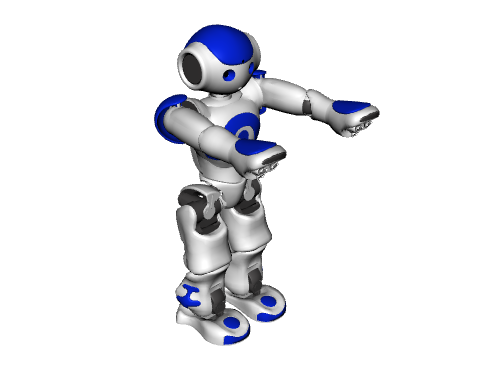
\includegraphics[width=0.5\textwidth]{figures/cap_3/modelo_original.png}
    \caption{Modelo del robot NAO utilizado}
    \label{fig:modelo_original}
\end{figure}

Este modelo\footnote{\url{https://app.gazebosim.org/OpenRobotics/fuel/models/NAO\%20with\%20Ignition\%20position\%20controller}} cuenta con un sistema de control de articulaciones ya construido, por lo que resulta perfecto para el proyecto. De hecho, el propio Gazebo Harmonic, al abrirse, tiene una demo que prueba este control de los joints de este mismo modelo, esto puede verse en la \autoref{fig:inicio_gazebo}.

Adjunto a continuación una captura de pantalla de dicha demostración (\autoref{fig:demo_gazebo}), así cómo un vídeo\footnote{\url{https://drive.google.com/file/d/1fe6DzpGnS2FQMr6UztVlayS8Wa_6vY5k/view?usp=sharing}} para que se aprecie bien el funcionamiento.

\begin{figure}[H]
    \centering
    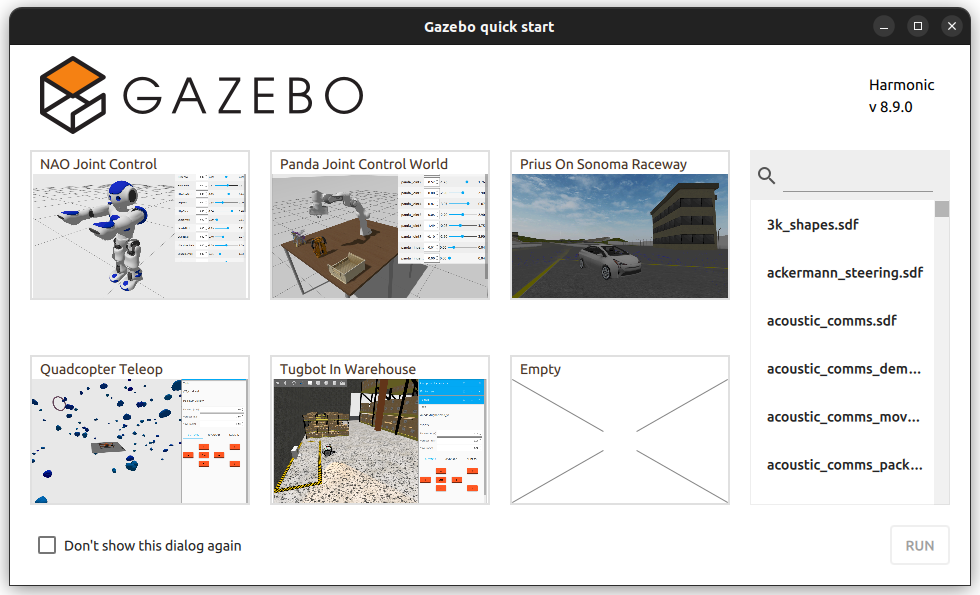
\includegraphics[width=1\textwidth]{figures/cap_3/inicio_gazebo.png}
    \caption{Inicio de Gazebo Harmonic, para acceder a la demo de control del NAO}
    \label{fig:inicio_gazebo}
\end{figure}

\begin{figure}[H]
    \centering
    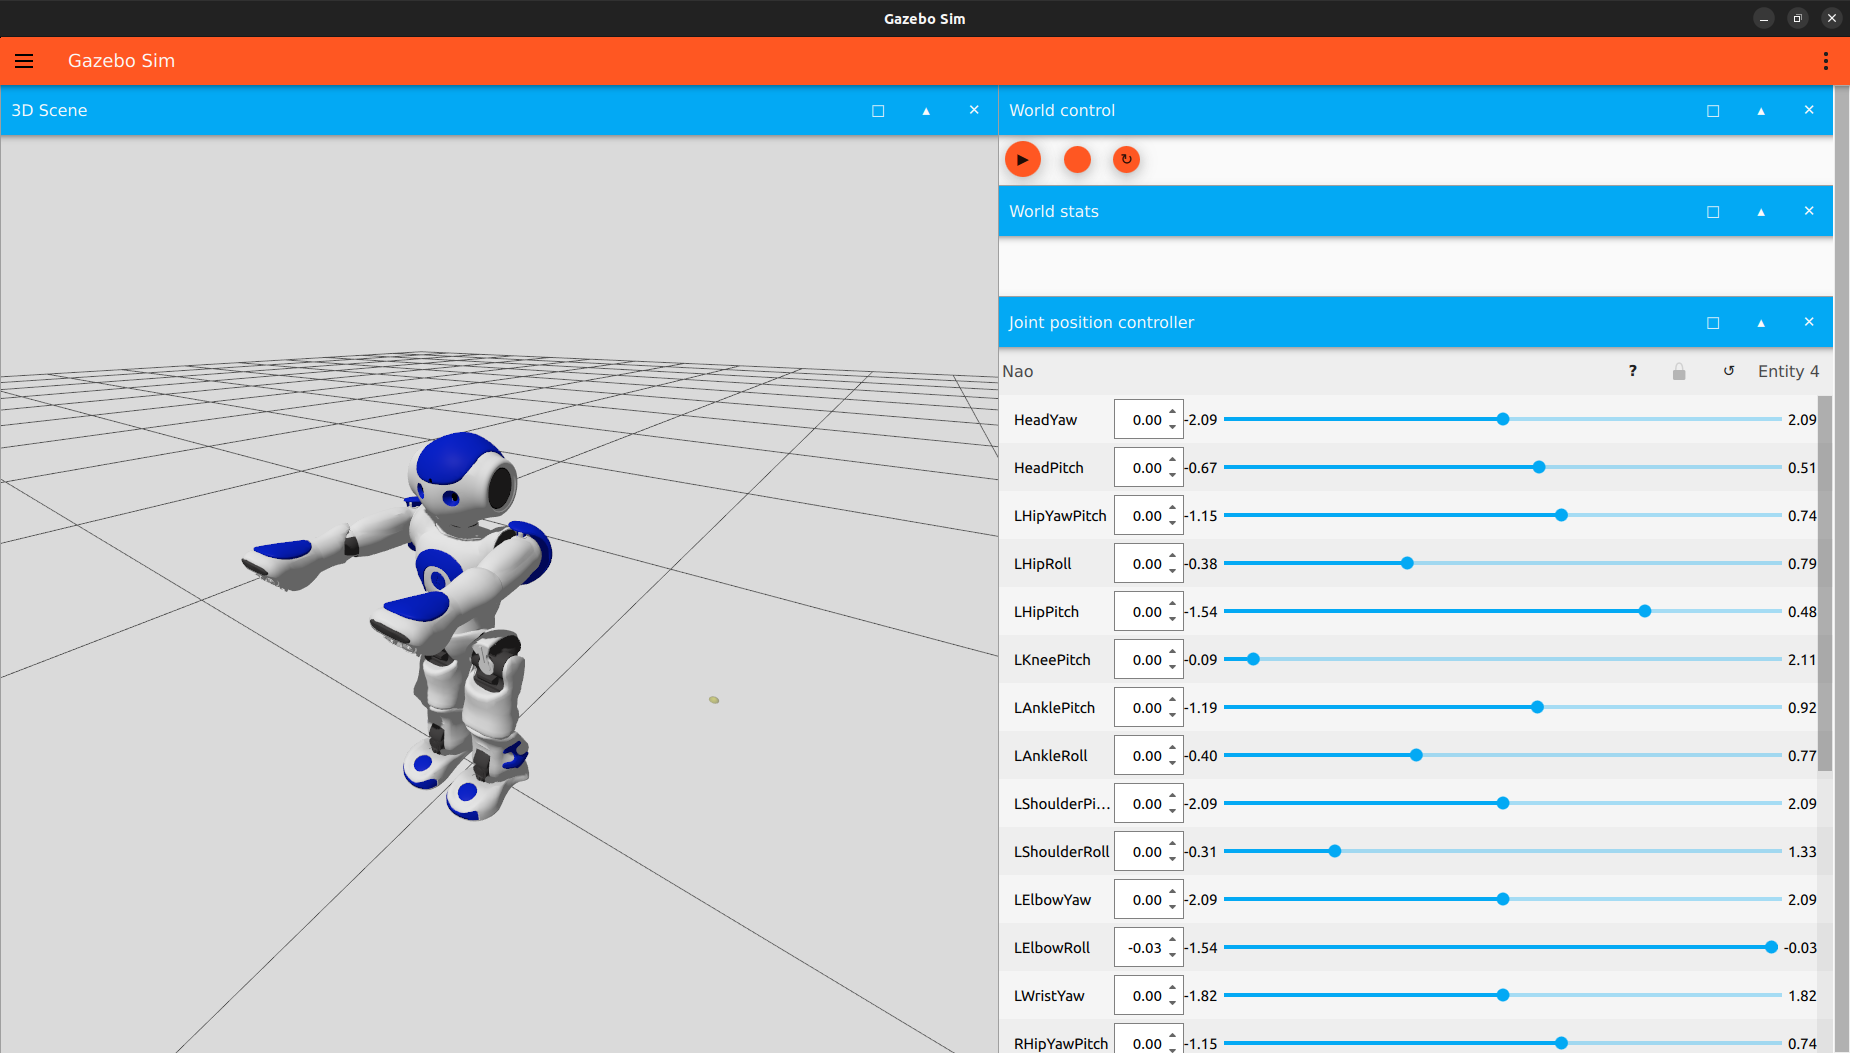
\includegraphics[width=1\textwidth]{figures/cap_3/demo_nao.png}
    \caption{Demo de Gazebo Harmonic para control de las articulaciones de NAO}
    \label{fig:demo_gazebo}
\end{figure}

El soporte básico de este modelo es ofrecer acceso a los actuadores de las articulaciones individualmente, sin embargo, no ofrece ningún mecanismo de coordinación o locomoción  que involucre a varias articulaciones de forma ordenada o coordinada. Pero el uso de Gazebo y este modelo en particular es necesario para probar los mecanismos de coordinación desarrollados en este TFG, y también para dotar al robot de un escenario para validar la aplicación robótica creada.

\section{Simulador Webots}

Webots\footnote{\url{https://cyberbotics.com/}} es una aplicación de escritorio multiplataforma de código abierto que se utiliza para simular robots. Proporciona un entorno de desarrollo completo para modelar, programar y simular robots.

Diseñado para uso profesional, se utiliza ampliamente en la industria, la educación y la investigación. Cyberbotics Ltd.\footnote{\url{https://es.linkedin.com/company/cyberbotics}} ha mantenido Webots como su producto principal desde 1998. Se muestra una imagen de una demo del robot NAO disponible en este simulador en la \autoref{fig:demo_webots}

\begin{figure}[H]
    \centering
    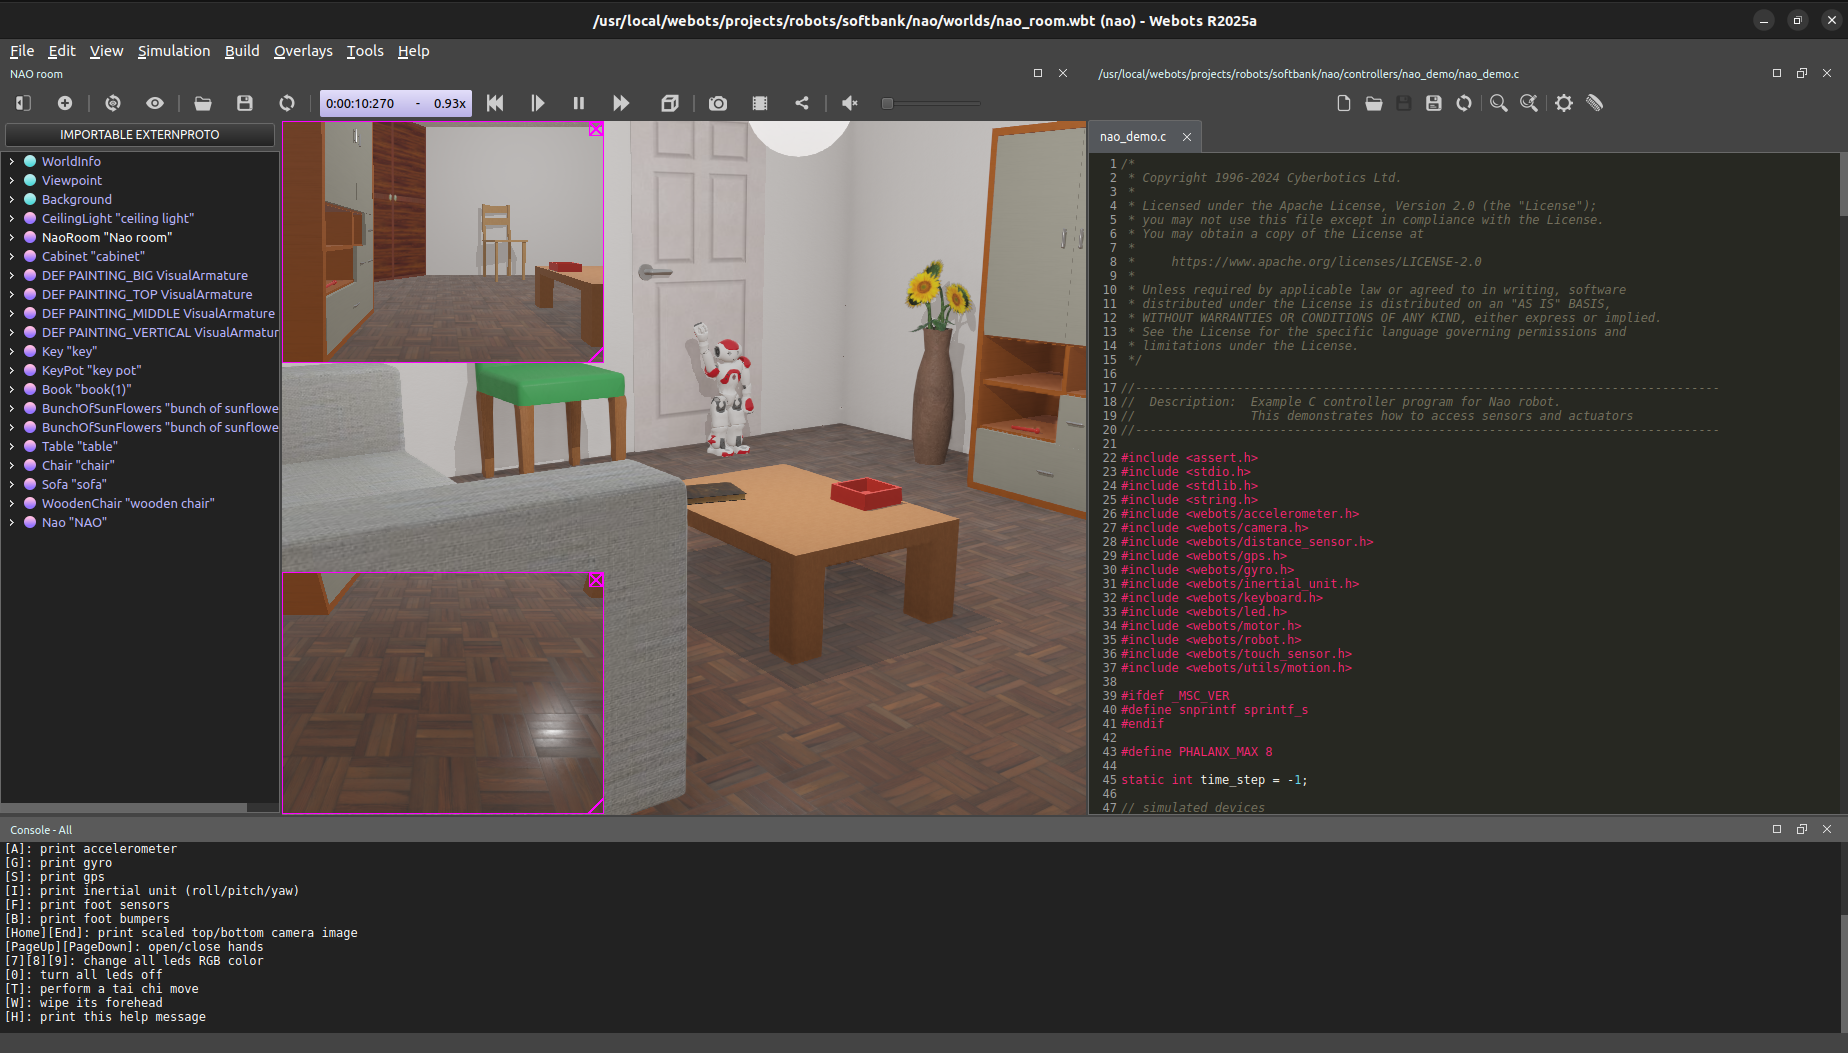
\includegraphics[width=1\textwidth]{figures/cap_3/webots.png}
    \caption{Demo de NAO en Webots}
    \label{fig:demo_webots}
\end{figure}

Se ha utilizado la versión R2025a, que, además de ser la más moderna, ya tiene resueltos patrones de movimiento del robot humanoide NAO que se han reciclado para el desarrollo de este TFG, los cuales son los siguientes:

\begin{itemize}
\item Caminar hacia adelante una secuencia de 10 pasos.
\item Caminar hacia atrás una secuencia de 2 pasos.
\item Levantarse del suelo si se ha caído boca abajo.
\item Caminar de forma lateral una secuencia de 2 pasos hacia la derecha.
\item Caminar de forma lateral una secuencia de 2 pasos hacia la izquierda.
\item Girar en el sitio hacia la derecha un ángulo de 40 grados.
\item Girar en el sitio hacia la derecha un ángulo de 60 grados.
\item Girar en el sitio hacia la izquierda un ángulo de 40 grados.
\item Girar en el sitio hacia la izquierda un ángulo de 60 grados.
\item Girar en el sitio hacia la izquierda un ángulo de 180 grados.
\end{itemize}

El uso de estos patrones y sus modificaciones se extenderá en el Capítulo~\ref{cap:capa_movimiento}.